\documentclass{article} % For LaTeX2e
% We will use NIPS submission format
\usepackage{nips13submit_e,times}
% for hyperlinks
\usepackage{hyperref}
\usepackage{url}
% For figures
\usepackage{graphicx} 
\usepackage{subfigure} 
% math packages
\usepackage{amsmath}
\usepackage{amsfonts}
\usepackage{amsopn}
\usepackage{ifthen}
\usepackage{natbib}

\title{Robust Fisher Linear Discriminant Analysis}

\author{
Jun Lu\\
EPFL \\
\texttt{jun.lu@epfl.ch} \\
}

% The \author macro works with any number of authors. There are two commands
% used to separate the names and addresses of multiple authors: \And and \AND.
%
% Using \And between authors leaves it to \LaTeX{} to determine where to break
% the lines. Using \AND forces a linebreak at that point. So, if \LaTeX{}
% puts 3 of 4 authors names on the first line, and the last on the second
% line, try using \AND instead of \And before the third author name.

\nipsfinalcopy 

\begin{document}

\maketitle

\begin{abstract}
In this report, we summarize our findings for the Robust Fisher LDA on the spring semester for the course of Convex Optimization and its Application.
\end{abstract}

\section{Data Description}
To demonstrate and compare the fisher LDA and robust fisher LDA, we used the sonar and ionosphere benchmark problems from the UCI repository (www.ics.uci.edu/~mlearn/MLRepository.html). The two benchmark problems have 208 and 351 points, respectively, and the dimension of each data point is 60 and 34, respectively.

\section{Fisher LDA}
Linear Discriminant Analysis (LDA) is most commonly used as dimensionality reduction technique in the preprocessing step for pattern classification and machine learning applications. The goal is to project a dataset onto a lower-dimensional space with good class-separability in order avoid overfitting (“curse of dimensionality”) and also reduce computational costs.

Let’s assume that our goal is to reduce the dimensions of a $d$-dimensional dataset by projecting it onto a $k$-dimensional subspace (where $k<d$). So, how do we know what size we should choose for $k$($k$ = the number of dimensions of the new feature subspace), and how do we know if we have a feature space that represents our data “well”?


We computed eigenvectors (the components) from our data set and collect them in a so-called scatter-matrices (i.e., the in-between-class scatter matrix and within-class scatter matrix).
Each of these eigenvectors is associated with an eigenvalue, which tells us about the “length” or “magnitude” of the eigenvectors.

If we would observe that all eigenvalues have a similar magnitude, then this may be a good indicator that our data is already projected on a “good” feature space.

And in the other scenario, if some of the eigenvalues are much much larger than others, we might be interested in keeping only those eigenvectors with the highest eigenvalues, since they contain more information about our data distribution. Vice versa, eigenvalues that are close to 0 are less informative and we might consider dropping those for constructing the new feature subspace.


\begin{figure}[h]
\center
\subfigure[sonar.]{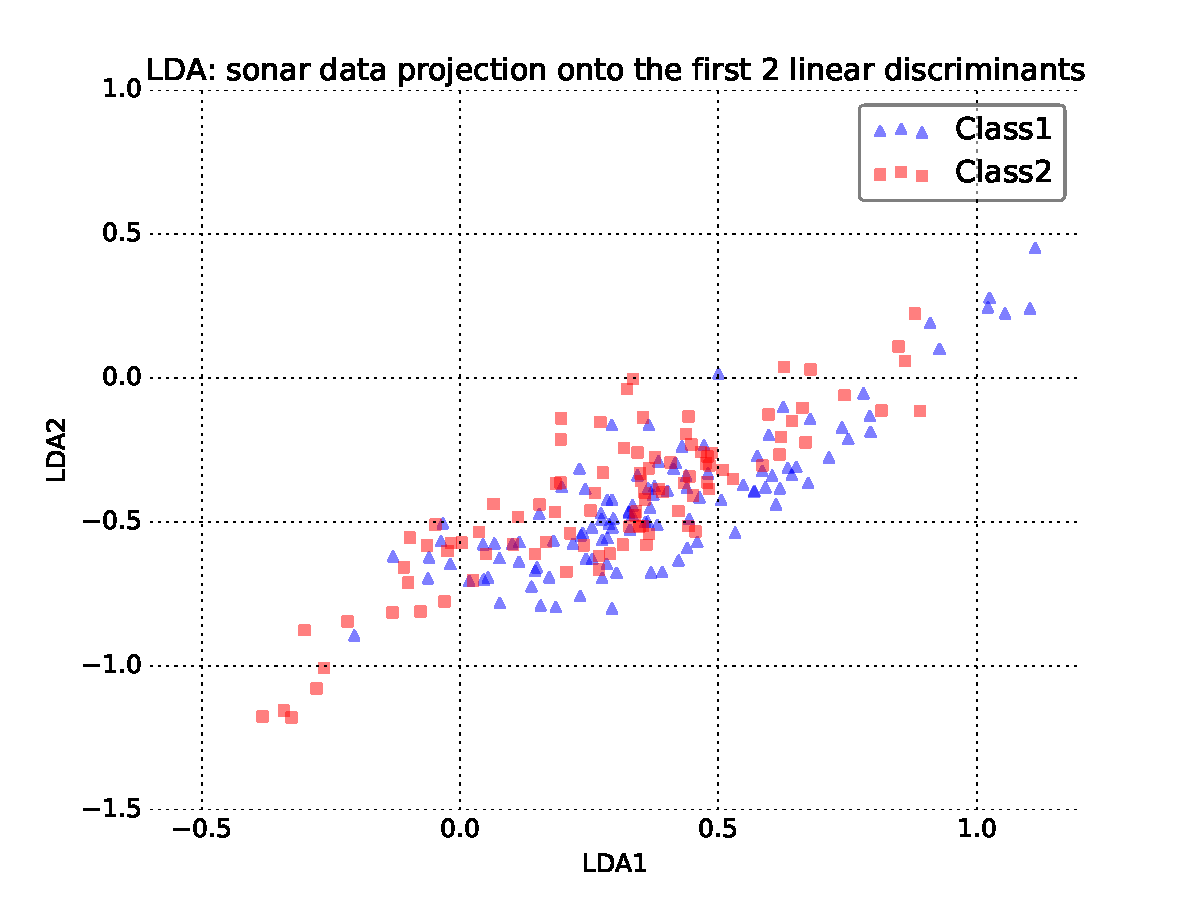
\includegraphics[width=2.6in]{figures/fishersonar.pdf} \label{fig:fishersonar}}
\hfill
\subfigure[ionosphere.]{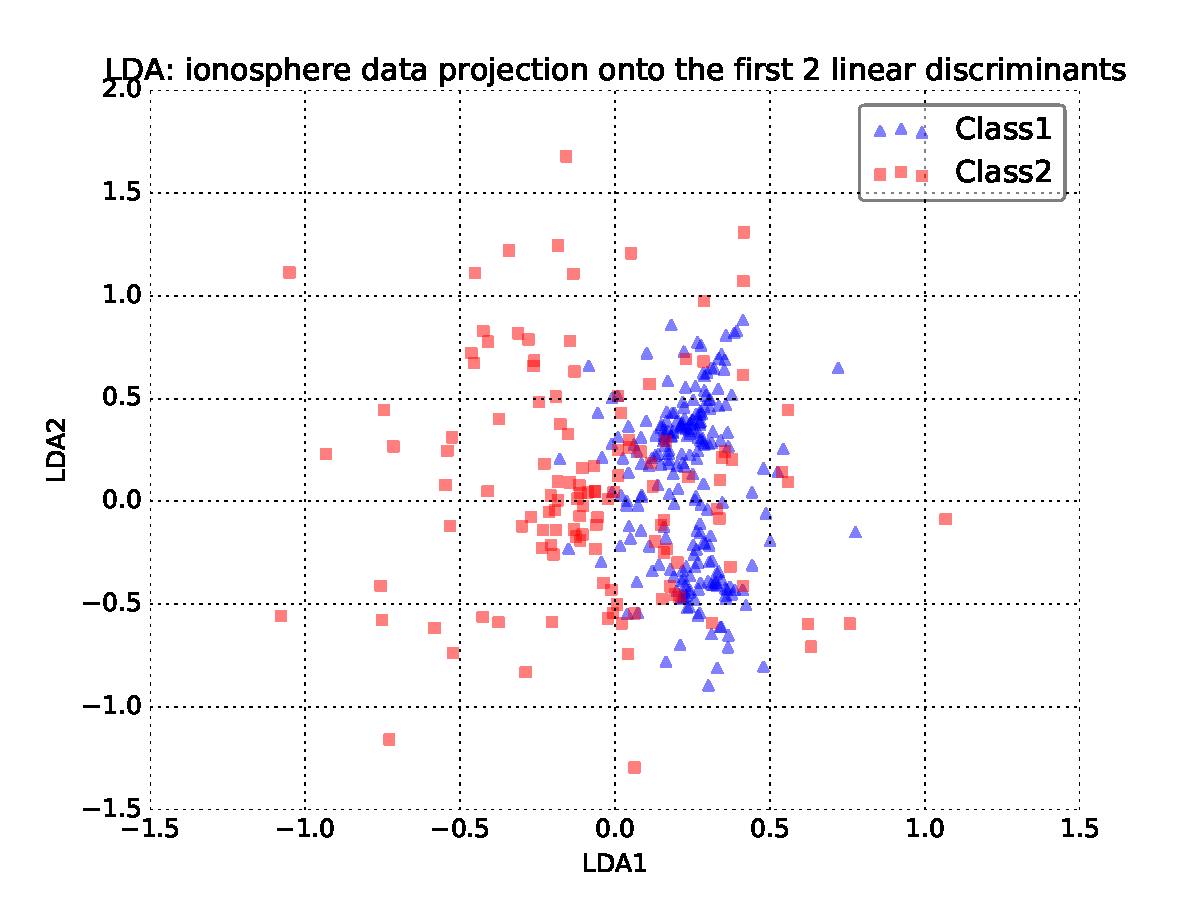
\includegraphics[width=2.6in]{figures/fisherionosphere.pdf} \label{fig:fisherionosphere}}
\caption{}
\end{figure}




\end{document}

